\section{Autonomous Forklift}
\label{sec:agv}
%
The mobile base is built upon a manual forklift which originally was equipped with motorized forks
and a drive wheel only. The forklift has been retrofitted with a steering mechanism and a commercial
AGV control system which is used to interface the original drive mechanism as well as the steering
servo. To assure safe operation, the vehicle is equipped with a SICK S300 safety laser
scanner\footnote{\url{http://www.sick.com/}} and an industrial prototype system for detecting human
workforce using reflective safety garments as described in Section~\ref{subsec:people_det}.
%
\subsection{Challenges in Autonomous Navigation}
\label{subsec:AGV_challenges}
%
The industry standard for autonomous navigation of forklifts is to use pre-defined trajectories
which are either manually defined or learned through teaching-by-demonstration from a human
operator~\cite{Hell06, Marsh08}. Although conceptually simple, pre-defining trajectories limits
pallet handling to occur only at pre-defined poses. In addition, only overly simple strategies for
handling unforeseen obstacles can be applied. The fundamental difficulties of motion planning for a
forklift lie in the nonholonomic constraints and the large sweep area it needs to occupy while
operating in a limited work space.

In order to obtain reliable localization in large dynamic warehouses with high accuracy, it is
common to mount reflectors in the environment and to use a dedicated sensing
device~\cite{Hyyp89}. This approach provides reliable navigation in smaller facilities where walls
are commonly observed. However, without additional infrastructure, navigation in large and dynamic
environments remains a challenge.
%
\subsection{Navigation}
\label{subsec:navigation}
%
The navigation module ensures that the forklift is capable of moving safely and autonomously through
the work space environment to arbitrary load/unload poses with high accuracy. According to the AGV
system provider Kollmorgen\footnote{\url{http://www.kollmorgen.com/}}, the required end pose
accuracy for picking up pallets is $\pm0.03$~m in position and $\pm1$~degree in orientation. The
navigation module comprises trajectory generation, tracking control and a localization system.
 
The online trajectory generation is done in two steps. First, a kinematically feasible path with
discretized start and goal poses is generated using a lattice planner~\cite{Ciri14}. Second, this
path is post-processed using a path smoother~\cite{Andr15} which assures a smooth, collision-free
and continuous trajectory, which allows to drive the vehicle with high accuracy. Subsequently, the
obtained trajectory is driven using a model predictive controller. For localization, a Velodyne
HDL-32 3D laser scanner\footnote{\url{http://www.velodynelidar.com/}} is utilized to construct a 3D
map (using the 3D-NDT-OM map representation) of the static parts of the
environment~\cite{Stoy13}. The map and odometry information is then used to localize the vehicle in
the presence of dynamic entities using a dual timescale approach~\cite{Vale14}. The complete
navigation system has been implemented, extensively tested and successfully integrated on the APPLE
demonstrator. A detailed description can be found in~\cite{Andr15}.

The current system for pallet detection and pickup requires a rough estimate of the location of the
pallet ($i.\,e.,$ a pre-defined pickup zone). In order to compute the final pose based on sensory
data from an Asus Xtion Pro Live\footnote{\url{http://www.asus.com/Multimedia/Xtion_PRO_LIVE/}}
mounted on the AGV, a Signed Distance Function (SDF) tracker~\cite{Cane13} is used with a pre-defined
SDF model of the pallet. The tracking is done while driving towards the pickup zone and the
trajectory is recomputed on the fly which, depending on the pose offset, may include a reverse
driving operation.
%
\subsection{Human Detection}
\label{subsec:people_det}
%
\begin{figure}[t!]
  \begin{center}
    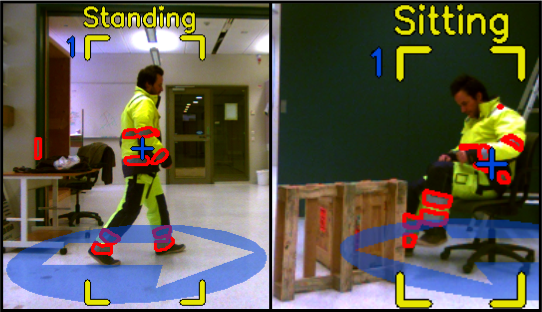
\includegraphics[width =0.99\linewidth]{figs/person_detection}
    % \vspace{-0.25cm}
    \caption{\textit{Human detection:} For safe navigation, the robot detects and tracks humans in
      the close neighborhood, estimates their position, and infers body pose information. Active
      infrared vision in combination with reflective safety clothing ensures robust performance
      independent of the illumination conditions.}
    \label{fig:people_det}
    \vspace{-0.55cm}
  \end{center}
\end{figure}
% 
As the envisioned mobile manipulation system will operate in environments shared with human
workforce, robust human detection is crucial to ensure a safe work environment. We address this
problem by using the recently developed RefleX workforce protection system~\cite{Mosb14}. RefleX is
a camera-based safety system designed for industrial vehicles and machinery, that detects and tracks
human workers wearing off-the-shelf high-visibility clothing (Fig.~\ref{fig:people_det}). Using
active near-infrared stereo vision, RefleX detects and locates the reflective markers on the safety
garments in order to estimate position and relative velocity of the observed person, and infer
further body pose information. The underlying sensing principle thereby ensures that the detection
performance is nearly independent of external illumination conditions. A classification of the
observed reflective patterns further allows the APPLE system to discriminate between a worker's
safety garments and other reflective navigation markers placed in the environment.
